\section{Optimointimenetelmät}

Tässä luvussa esitellään muutamia menetelmiä, joilla kehittäjät ovat parantaneet virtuaalikoneidensa tuottaman konekoodin suorituskykyä. Osa menetelmistä hyödyntää virtuaalikoneen keräämää tietoa sovelluksessa esiintyvistä tyypeistä.

%Konekoodin suorittaminen on nopeaa, mutta kääntäminen on hidas prosessi varsinkin, jos kääntäjä tekee monimutkaisia optimointeja. Tämän takia modernit virtuaalikoneet sisältävät useamman kuin yhden JIT-kääntäjän, kuten esimerkiksi V8:n tapauksessa. Tässä luvussa esitellään muutamia menetelmiä, joilla kehittäjät ovat parantaneet virtuaalikoneidensa tuottaman konekoodin suorituskykyä.

\subsection{Piiloluokat}

JavaScriptin oliot käyttävät prototyyppiperintää. Tämä tarkoittaa, että oliolla on käytännössä aina jokin olio prototyyppinään, jolla on toinen olio prototyyppinään ja niin edelleen. Kun oliolta pyydetään jonkin \textit{ominaisuuden} (property) arvoa, etsitään sitä ensin itse oliosta. Jos ominaisuutta ei löydy, käydään olion prototyyppiketjua läpi, kunnes se löytyy tai kaikki prototyypit on käyty läpi, jolloin ominaisuuden arvoksi palautetaan \texttt{undefined}.

Ominaisuuden lisääminen tai muuttaminen päivittää oliota, ei koskaan sen prototyyppiä. Jos ominaisuutta ei ole oliossa, se lisätään siihen, vaikka kyseinen ominaisuus löytyisikin prototyyppiketjusta. Tällöin saman prototyypin omaavat oliot säilyttävän vanhan arvon ja vain muutettu olio käyttää uutta arvoa. Olion prototyyppiä pääsee kuitenkin muokkaamaan epästandardin \texttt{\_\_proto\_\_}-ominaisuuden kautta tai standardiin myöhemmin lisätyn \texttt{Object.getPrototypeOf(obj)}-funktion avulla.

Dynaamisesta prototyyppiperintämallista johtuen ominaisuuksien arvot saattavat olla muistissa kaukana toisistaan ja niiden löytämiseen tarvitaan hidasta assosiatiivista hakurakennetta. Staattisissa luokkaperintään pohjautuvissa kielissä olioiden rakenne on helppo muuttaa tietokoneen ymmärtämään muotoon.

V8:n kehittäjät esittelivät ominaisuuden nimeltään \textit{piiloluokka} (hidden class)~\cite{v8design}. Piiloluokat ovat \textit{muuttumattomia} (immutable) luokkia, joita virtuaalikone käyttää JavaScript-olioiden rakenteen kuvaamiseen. Piiloluokka on tavallaan siis olion tyyppi, vaikka JavaScriptissä olioilla ei ole varsinaisesti tyyppejä, paitsi kieleen sisäänrakennetut perustyypit, kuten \texttt{String} ja \texttt{Number}. Käyttämällä piiloluokkaa olion tyyppinä virtuaalikoneet voivat hyödyntää tehokkaita kääntämistekniikoita, joita käytetään yleisesti staattisesti tyypitetyissä kielissä.

Piiloluokat toimivat siten, että oliota luodessa ensimmäistä kertaa, virtuaalikone luo sille samalla piiloluokan. Aina kun oliota muutetaan lisäämällä siihen ominaisuus, luodaan sitä vastaamaan uusi piiloluokka tai käytetään olemassa olevaa piiloluokkaa. Piiloluokkia ei voi tehdä etukäteen, koska dynaamisuuden takia on vaikea tietää ennalta millainen olio tulee rakenteeltaan olemaan. 

Kuvassa~\ref{fig:hiddenclass} näkyy, miten V8 luo piiloluokkia luodessaan Piste-olion ensimmäisen kerran. Jokainen kaavion askel vastaa yhden koodirivin suorittamista. Kun konstruktorifunktiota kutsutaan, luodaan tyhjä olio, johon viitataan avainsanalla \texttt{this}. Virtuaalikone kuvaa sitä tyhjällä piiloluokalla \texttt{C0}. Luokkaa \texttt{C0} käytetään kuvaamaan kaikkia tyhjiä olioita, joilla on sama prototyyppi, joka on oletuksena kieleen sisäänrakennetun \texttt{Object}-olion ilmentymä. Konstruktorissa olioon liitetään ominaisuus \texttt{x}, jolloin virtuaalikone luo uuden piiloluokan \texttt{C1} ja lopulta \texttt{y}:n lisäyksen jälkeen \texttt{C2}:n. Piiloluokkiin tallennetaan myös tieto mihin luokkaan pitää siirtyä tietyn ominaisuuden lisäämisen jälkeen sekä viittaus olion prototyyppiin.

\begin{figure}[ht]
    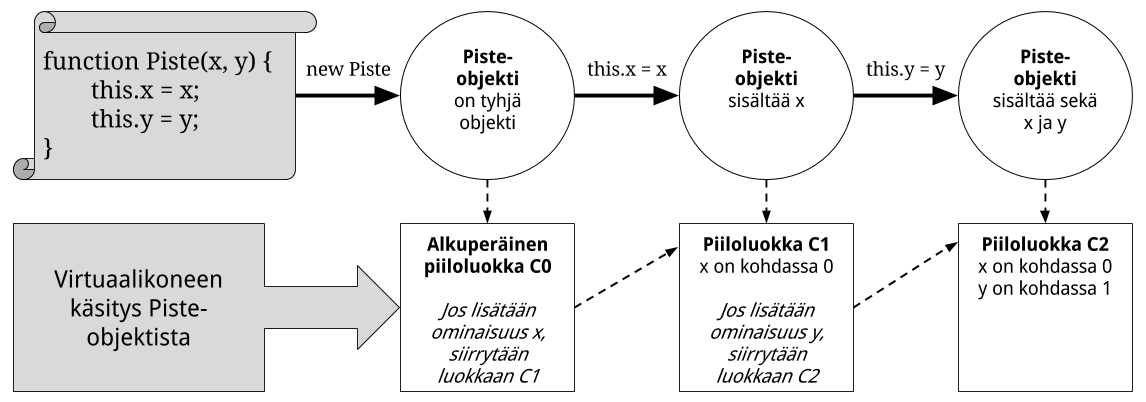
\includegraphics[width=\textwidth]{hidden-classes}
    \caption{Esimerkki piiloluokkien toimintaperiaatteesta.}
     \centering
     \label{fig:hiddenclass}
\end{figure}

Piiloluokkia ei tarvitse luoda uudestaan joka kerta, kun halutaan luoda uusi Piste-olio. Riittää, että seurataan niihin sisällytettyjä tietoja siirtymistä. Kun uusi Piste-olio luodaan, päädytään lopulta samaan piiloluokkaan \texttt{C2}. Kaikki Piste-oliot ovat siis virtuaalikoneen näkökulmasta samantyyppisiä.

Kun Piste-oliolta pyydetään esimerkiksi ominaisuuden \texttt{x} arvoa, virtuaalikone tietää, että olio on luokan \texttt{C2} ''tyyppinen'' ja arvo löytyy yhdellä konekäskyllä olion muistipaikasta siirtymällä 0 ilman, että täytyy tehdä hidasta hakua assosiatiivisesta hakurakenteesta. Virtuaalikone voi siis generoida tehokkaampaa konekoodia ja muistiviittaukset nopeutuvat huomattavasti.

%Jos oliota muokataan luomisen jälkeen, luodaan sille uusi piiloluokka ja optimoinnit täytyy suorittaa tälle uudelle tyypille uudestaan. Jos kaikkia ominaisuuksia ei alusteta aina samassa järjestyksessä tai niitä alustetaan ehdollisesti, se tuottaa ongelmia piiloluokkien toiminnan kannalta.

Syy, miksi luodaan useita piiloluokkia yhden olion luonnin yhteydessä on, että niihin lisätyt siirtymätiedot mahdollistavat erilaisten olioiden luomisen käyttäen hyväksi jo luotuja piiloluokkia. Esimerkiksi \texttt{Ympyrä}-olio voi sisältää ominaisuudet \texttt{x}, \texttt{y} ja \texttt{r}, jolloin sen luomisessa käytetään piiloluokkia \texttt{C0}, \texttt{C1}, \texttt{C2} ja luodaan uusi \texttt{C3}. Vaihtoehtoisesti voimme luoda 3-ulotteisen Pisteen, jolla on tasokoordinaattien lisäksi \texttt{z}-ominaisuus. Tällöin piiloluokka \texttt{C2} sisältää tiedon siirtymästä molemmissa, ympyrän ja 3-ulotteisen pisteen, tapauksissa.

Wonsun Ahn kumppaneineen on tutkinut piiloluokkien hyötyjä ja haittoja todellisissa verkkosovelluksissa~\cite{Ahn2014}. Tutkimuksissa on löytynyt muutamia heikkouksia, jotka vähentävät piiloluokkien hyötyjä todellisissa sovelluksissa ja heikkouksiin ehdotetaan parannuksia. Tutkimuksessa myös moititaan kehittäjien vahvaa oletusta ohjelmien staattisesta käytöksestä.

\subsection{Sisällytetty välimuisti}

\textit{Hakupaikaksi} (access site) kutsutaan kohtaa koodissa, jossa viitataan olion ominaisuuteen. Koska muuttujilla ei ole tyyppiä, virtuaalikone ei voi tietää ennalta löytyykö edes kyseistä ominaisuutta. Yleinen olettamus on, että samalla hakupaikalla oliot ovat usein samantyyppisiä. Tämän takia esimerkiksi V8:ssa on alettu käyttää \textit{sisällytettyä välimuistia} (inline cache)~\cite[s.~498]{Ahn2014}. Nimi tulee siitä, että välimuisti on osa generoitua konekoodia.

Olkoon esimerkiksi funktio \texttt{getX(obj)}, joka palauttaa sille syötetyn olion ominaisuuden \texttt{x} arvon. Keräämällä tietoa suoritusaikana virtuaalikone voi päätellä, että tässä hakupaikassa \texttt{obj} on usein Piste-olio. Virtuaalikone voi muokata konekoodia ja lisätä tarkistuksen: ''Onko \texttt{obj}:n piiloluokka \texttt{C2}?'' Jos oliolla on tämä piiloluokka, arvon lukemiseksi riittää katsoa piiloluokasta sen siirtymä muistissa ja suorittaa yksi konekäsky sen hakemiseksi.

V8:ssa on kolmen tyyppisiä sisällytettyjä välimuisteja: \textit{lataukselle} (load), \textit{talletukselle} (store) ja \textit{kutsumiselle} (call). Lataaminen tarkoittaa olion ominaisuuden hakemista ja talletus sen päivittämistä. Kutsuminen tarkoittaa olioon liitetyn funktion kutsumista ja se on samankaltainen lataamisen kanssa, sillä ensin pitää ladata funktio, joka on JavaScriptissä viittaus funktio-olioon.

Jos olion tyyppiä ei löydy sisällytetystä välimuistista, V8 voi lisätä tarkistuksen sisällytettyyn välimuistiin. Esimerkiksi jos ohjelma alkaa kutsua \texttt{getX}-funktiota ympyräolioilla, V8 voi lisätä sisällytettyyn välimuistiin tarkistuksen: ''Onko \texttt{obj}:n piiloluokka \texttt{C3}?'', jolloin arvon voi ladata taas nopeasti tunnetusta siirtymästä. Tämä vaatii muutoksia suorituksessa olevaan konekoodiin, koska sisällytetty välimuisti on osa konekoodia.

Ylimääräiset tarkistukset tekevät suorituksesta hitaampaa. Tutkimuksen mukaan suoritus välimuistin avulla voi olla parhaimmillaan monta kertaluokkaa nopeampaa kuin ilman välimuistia~\cite[s.~498]{Ahn2014}, joten  tulokset tukevat sisällytetyn välimuistin käyttöä.

\subsection{Aktivaatiotietueiden manipulointi}

(On-stack replacement)

\subsection{Roskienkeruu}

JavaScript-virtuaalikoneiden \textit{roskienkeruu} (garbage collection) on perinteisesti toiminut melko yksinkertaisella algoritmilla nimeltään \textit{merkitse ja pyyhkäise} (mark-and-sweep). Algoritmi perustuu nimensä mukaisesti kahteen vaiheeseen. Ensimmäinen on merkitsemisvaihe, jossa käydään läpi kaikki ohjelman viittaamat oliot ja merkitään ne. Sitten seuraa pyyhkäisyvaihe, jossa koko muisti käydään läpi ja vapautetaan kaikki oliot, jotka eivät ole merkittyjä ja samalla poistetaan merkit seuraavaa suoritusta varten.

Ohjelman suoritus ei voi jatkua roskienkeruun aikana, koska ohjelma voi käyttää muistia milloin vain, ja koko muistialueen käsitteleminen on hidasta. Tämä on suuri ongelma varsinkin animaatioiden ja interaktiivisten sovellusten tapauksessa, sillä pitkä roskienkeruutauko haittaa käytettävyyttä ja saa sovelluksen tuntumaan hitaalta, vaikka muu suoritus olisikin todella nopeaa.

Ongelman ratkaisemiseksi on kehitetty monenlaisia heuristiikkoja ja optimointeja. Automaattisesta muistinhallinnasta riittää materiaalia useampaankin tutkielmaan~\cite{gcbib}, joten on listaan tässä tärkeimpiä menetelmiä, joilla roskienkeruuta on parannettu:

\begin{itemize}
\item \textit{sukupolvittainen roskienkeruu} (generational garbage collection)~\cite{v8design}
\item \textit{inkrementaalinen roskienkeruu} (incremental garbage collection)~\cite{incrementalgc}
\item roskienkeruu ''luppoaikana'' eli roskienkeruun aikataulutus~\cite{freegc}
\item \textit{lehtioliot} (leaf objects) eli oliot joista ei lähde viittauksia~\cite{ie10}
\end{itemize}

%\subsection{Staattinen kertasijoitusmuoto}

%(Static single assignment form, SSA)

%https://blog.chromium.org/2010/12/new-crankshaft-for-v8.html
%An optimizing compiler which recompiles and optimizes hot code identified by the runtime profiler. It uses static single assignment form to perform optimizations such as loop-invariant code motion, linear-scan register allocation and inlining. The optimization decisions are based on type information collected while running the code produced by the base compiler.